% Figure: Segment structure diagram
\begin{figure}[h]
\centering
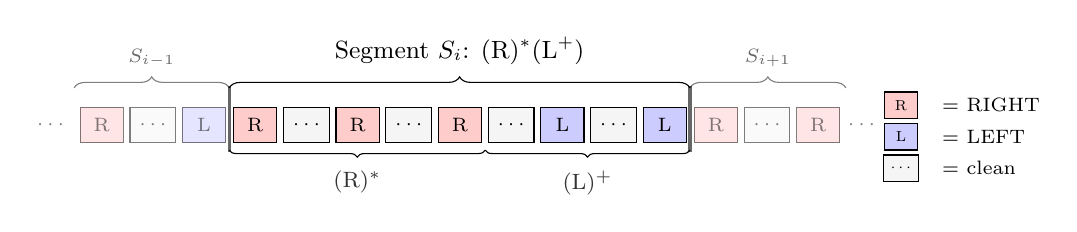
\begin{tikzpicture}[
    cell/.style={minimum width=0.55cm, minimum height=0.45cm, draw, font=\scriptsize},
    dotcell/.style={minimum width=0.45cm, minimum height=0.45cm, font=\scriptsize},
    right/.style={cell, fill=red!20},
    left/.style={cell, fill=blue!20},
    clean/.style={cell, fill=gray!8},
    boundary/.style={very thick, black!60},
    segbrace/.style={decorate, decoration={brace, amplitude=4pt}},
    subbrace/.style={decorate, decoration={brace, amplitude=2.5pt, mirror}},
    seglabel/.style={font=\footnotesize, text=black!80},
    faded/.style={opacity=0.5}
]

% === PREVIOUS SEGMENT (faded) ===
\begin{scope}[faded]
  \node[dotcell] at (-1.3, 0) {$\cdots$};
  \node[right] (pr1) at (-0.65, 0) {R};
  \node[clean] at (0, 0) {$\cdots$};
  \node[left] (pl1) at (0.65, 0) {L};
\end{scope}

% Boundary: previous segment | current segment
\draw[boundary] (0.97, 0.5) -- (0.97, -0.35);

% === CURRENT SEGMENT (main focus) ===
% RIGHT region: R [...] R [...] R
\node[right] (r1) at (1.3, 0) {R};
\node[clean] at (1.95, 0) {$\cdots$};
\node[right] (r2) at (2.6, 0) {R};
\node[clean] at (3.25, 0) {$\cdots$};
\node[right] (r3) at (3.9, 0) {R};

% LEFT region: [...] L [...] L
\node[clean] at (4.55, 0) {$\cdots$};
\node[left] (l1) at (5.2, 0) {L};
\node[clean] at (5.85, 0) {$\cdots$};
\node[left] (l2) at (6.5, 0) {L};

% Boundary: current segment | next segment
\draw[boundary] (6.82, 0.5) -- (6.82, -0.35);

% === NEXT SEGMENT (faded) ===
\begin{scope}[faded]
  \node[right] (nr1) at (7.15, 0) {R};
  \node[clean] at (7.8, 0) {$\cdots$};
  \node[right] (nr2) at (8.45, 0) {R};
  \node[dotcell] at (9.0, 0) {$\cdots$};
\end{scope}

% === ANNOTATIONS ===
% Main segment brace (top)
\draw[segbrace] (0.97, 0.47) -- (6.82, 0.47) 
    node[midway, above=5pt, font=\small] {Segment $S_i$: $(\mathrm{R})^*(\mathrm{L}^+)$};

% Sub-braces (bottom)
\draw[subbrace] (0.97, -0.32) -- (4.22, -0.32) 
    node[midway, below=4pt, seglabel, align=center] {$(\mathrm{R})^*$};
\draw[subbrace] (4.22, -0.32) -- (6.82, -0.32) 
    node[midway, below=4pt, seglabel, align=center] {$(\mathrm{L})^+$};

% Adjacent segment labels (above, smaller)
\draw[segbrace, faded] (-1.0, 0.47) -- (0.97, 0.47) 
    node[midway, above=4pt, font=\scriptsize, opacity=0.6] {$S_{i-1}$};
\draw[segbrace, faded] (6.82, 0.47) -- (8.8, 0.47) 
    node[midway, above=4pt, font=\scriptsize, opacity=0.6] {$S_{i+1}$};

% Legend
\node[right, scale=0.75] at (9.5, 0.25) {R};
\node[font=\scriptsize, anchor=west] at (9.9, 0.25) {= RIGHT};
\node[left, scale=0.75] at (9.5, -0.15) {L};
\node[font=\scriptsize, anchor=west] at (9.9, -0.15) {= LEFT};
\node[clean, scale=0.75] at (9.5, -0.55) {$\cdots$};
\node[font=\scriptsize, anchor=west] at (9.9, -0.55) {= clean};

\end{tikzpicture}
\caption{Segment structure after Phase~1. Each segment follows the pattern $(\mathrm{R})^*(\mathrm{L}^+ \mid \epsilon)$: zero or more RIGHT violations followed by one or more LEFT violations.}
\label{fig:segment-diagram}
\end{figure}
